\documentclass[crop=true,tikz,border=1pt,varwidth=8in]{standalone}

%\makeatletter
%%%%%%%%%%%%%%%%%
\PassOptionsToPackage{force}{filehook}
\usepackage{tikz}
\usetikzlibrary{shapes,arrows}
\usetikzlibrary{positioning}
\tikzstyle{cloud} = [draw, ellipse,fill=red!20, node distance=0.87cm,
minimum height=2em]
\tikzstyle{line} = [draw, -latex', color=yellow]
\usetikzlibrary{shapes.symbols,shapes.callouts,patterns}
\usetikzlibrary{calc}


\begin{document}
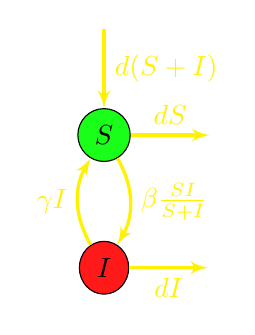
\begin{tikzpicture}[auto, %node distance = 2cm, auto,
	cloud/.style={minimum width={width("N-1")+2pt},
		draw, ellipse,fill=red!20}]
	\node [cloud, fill=green!90] (S) {$S$};
	\node [cloud, below=of S, fill=red!90] (I) {$I$};
	\coordinate[above=of S] (h1);
	\coordinate[right=of S] (h2);
	\coordinate[right=of I] (h3);
	%% Flows
	\path [line, bend left, very thick] (S) to node [midway, right] (TextNode) {$\beta\frac{SI}{S+I}$} (I);
	\path [line, bend left, very thick] (I) to node [midway, left] (TextNode) {$\gamma I$} (S);
	\path [line, very thick] (h1) to node [midway, right] (TextNode) {$d(S+I)$} (S);
	\path [line, very thick] (S) to node [midway, above] (TextNode) {$dS$} (h2);
	\path [line, very thick] (I) to node [midway, below] (TextNode) {$dI$} (h3);
\end{tikzpicture}
\end{document}